\chapter{What COMSOL really computes}\label{ch:comsol}

This chapter covers 13 and 14 November. It answers a question that had been open since 1 November, and its answer
decided how the 10\um\ work was done.

\section{The puzzle}

Our simulator draws wires and computes their field with exact physics. Close to the coil it agreed with COMSOL to
within the mesh noise. Higher up it drifted away, and at 10\um\ it was off by 65\%, 61\% and 134\% for $B_x$, $B_y$ and
$B_z$. Either our physics was wrong, or COMSOL's was. On 13 November Hari sent the COMSOL model files: the full
reports, the coil drawing, and exports on a second, finer mesh. Everything below was computed from them by the
scripts in \code{scripts/comsol_check/}. Nothing was trained.

\section{The model}

\begin{center}
\small
\begin{tabularx}{\textwidth}{>{\raggedright\arraybackslash}p{3.2cm}X}
\toprule
Item & In the COMSOL model \\
\midrule
Physics & Magnetic Fields, a \emph{stationary} study: nothing changes in time \\
Domain & One block of air, $140\times140\times90$\um \\
Walls & ``Magnetic insulation'' on all six faces: no field line may cross a wall \\
Coil & Wires 2.00\um\ wide, carrying 600\,\textmu A, as a sheet of zero thickness at $z=0$ \\
Leads & They run to the wall; the current returns through the wall \\
One solve for four data sets & \code{L1_C1} and the three multi-coil sets come from the same model and mesh \\
Mesh & 284{,}696 tetrahedra (``Extra Fine''), and a second export on 1{,}372{,}173 (``Extremely Fine'') \\
Export & A cut plane at each height, $1400\times1400$ points at 0.1\um \\
\bottomrule
\end{tabularx}
\end{center}

Two facts in this table already explain old observations. The four C1 configurations share one solve, so they share
their mesh noise (Chapter~\ref{ch:review}). And the exported window is the \emph{whole} box, wall to wall.

\section{First check: the quarter turn}

Since October the code had rotated COMSOL's components by a quarter turn, because it made the data look right. Now the
reason is known. The columns \code{cpl1x} and \code{cpl1y} of the export are the cut plane's own axes, and COMSOL turned
them against the model's axes. The field columns are in the model's axes. So along the image axes, the components are

\begin{code*}{comsol_check/decay_rate.py}
def frame(B):
    Bx, By, Bz = B.astype(float); return -By, Bx, Bz
\end{code*}

How do we know this is right and not just convenient? With the test of Chapter~\ref{ch:limits}: the three components of
a real field are tied together. With this mapping the tie holds to 6\%. With the naive labels it fails completely
(100\%).

\section{Second check: the walls are there, but they are not the cause}

A closed box with insulating walls leaves fingerprints. The field component pointing into each wall should vanish,
and it does: 0.2--0.6\% of the typical field at the window edges. The average of $B_z$ over a plane should be zero, and
it is, to four decimals at every height.

Our simulator has no walls. It pads with zeros, as if space went on forever. Is that the problem? No. Propagating
COMSOL's own 0.5\um\ field up to 10\um\ with an exact model of the box (mirror images in every wall) misses COMSOL's
10\um\ field by 50.1\%. Without walls it misses by 50.8\%. The walls change almost nothing.

\section{Measuring how fast the field really decays}\label{sec:cm_decay}

So measure the decay directly. Physics says: between two heights $\Delta z$ apart, a ripple of frequency $k$ shrinks by
$e^{-k\,\Delta z}$. Take two COMSOL planes, look at one band of frequencies in both, and ask by what factor it shrank.
The decay rate is minus the logarithm of that factor, divided by $\Delta z$. If COMSOL obeys physics, the rate equals
$k$.

\begin{code*}{comsol_check/decay_rate.py}
    for lo, hi in bands:
        m = (K >= lo) & (K < hi)
        num = sum(np.vdot(a[m], b[m]) for a, b in zip(F1, F2))
        den = sum(np.vdot(a[m], a[m]) for a in F1)
        r = (num/den).real
        kc = np.sqrt(np.mean(K[m]**2))
        out.append((kc, -np.log(max(r, 1e-12))/dz))
\end{code*}

\code{F1} and \code{F2} are the spectra of the lower and the upper plane. \code{num/den} is the least-squares factor
between them in that band, over all three components. The last line turns it into a rate.

\begin{center}
\small
\begin{tabular}{lccccccc}
\toprule
Band $k$ (rad/\um) & 0.027 & 0.075 & 0.109 & 0.155 & 0.216 & 0.303 & 0.432 \\
\midrule
Physics predicts: rate $=k$ & 0.027 & 0.075 & 0.109 & 0.155 & 0.216 & 0.303 & 0.432 \\
Measured, 0.5 to 3\um & 0.103 & 0.128 & 0.144 & 0.189 & 0.240 & 0.329 & 0.445 \\
Measured, 3 to 6\um & 0.104 & 0.126 & 0.141 & 0.187 & 0.238 & 0.327 & 0.435 \\
Measured, 6 to 10\um & 0.106 & 0.127 & 0.141 & 0.188 & 0.237 & 0.329 & 0.420 \\
\midrule
$\sqrt{k^2+0.10^2}$ & 0.104 & 0.125 & 0.148 & 0.184 & 0.238 & 0.319 & 0.443 \\
\bottomrule
\end{tabular}
\end{center}

\begin{keyidea}[What the table says]
At the lowest frequency COMSOL's field decays almost \emph{four times} faster than physics allows (0.103 against
0.027). The excess is the same at every height, and one formula fits every band:
\[
\text{rate}=\sqrt{k^2+k_0^2},\qquad k_0\approx0.10\ \text{rad/\um}.
\]
For fine detail ($k\gg k_0$) the extra term does not matter. For broad structure it dominates.
\end{keyidea}

That is why the problem only shows at large standoffs. At 0.5\um\ only 11\% of the field lies below $k=0.1$\,rad/\um. At
10\um, where everything fine has already died away, 70\% of it does.

\section{One constant closes the gap}

If this is the whole story, then putting $k_0$ into our own model should make it match COMSOL. Starting from the exact
coil drawing:

\begin{center}
\footnotesize
\setlength{\tabcolsep}{4pt}
\begin{tabular}{lccc}
\toprule
Ours against COMSOL, $B_x$ / $B_y$ / $B_z$ & Free space & Box walls & Walls and $k_0=0.10$ \\
\midrule
at 3\um & 14.0 / 12.0 / 24.7\% & 14.0 / 13.0 / 25.1\% & 11.0 / 10.5 / 10.9\% \\
at 5\um & 23.2 / 19.9 / 45.9\% & 23.1 / 21.4 / 45.7\% & 11.3 / 11.6 / 12.3\% \\
at 10\um & 64.9 / 60.5 / 134.2\% & 64.5 / 57.7 / 128.9\% & \textbf{10.1 / 11.8 / 12.4\%} \\
\bottomrule
\end{tabular}
\end{center}

With $k_0$ the mismatch is 10--12\% at every height, and that is about the size of COMSOL's own mesh noise. The amplitude
comes out right too (scale 1.00). On a configuration that was not used to find $k_0$ (all four coils, at 12.5\um) the
mismatch falls from 83 / 75 / 66\% to 10 / 11 / 10\%.

\begin{figure}[H]
\centering
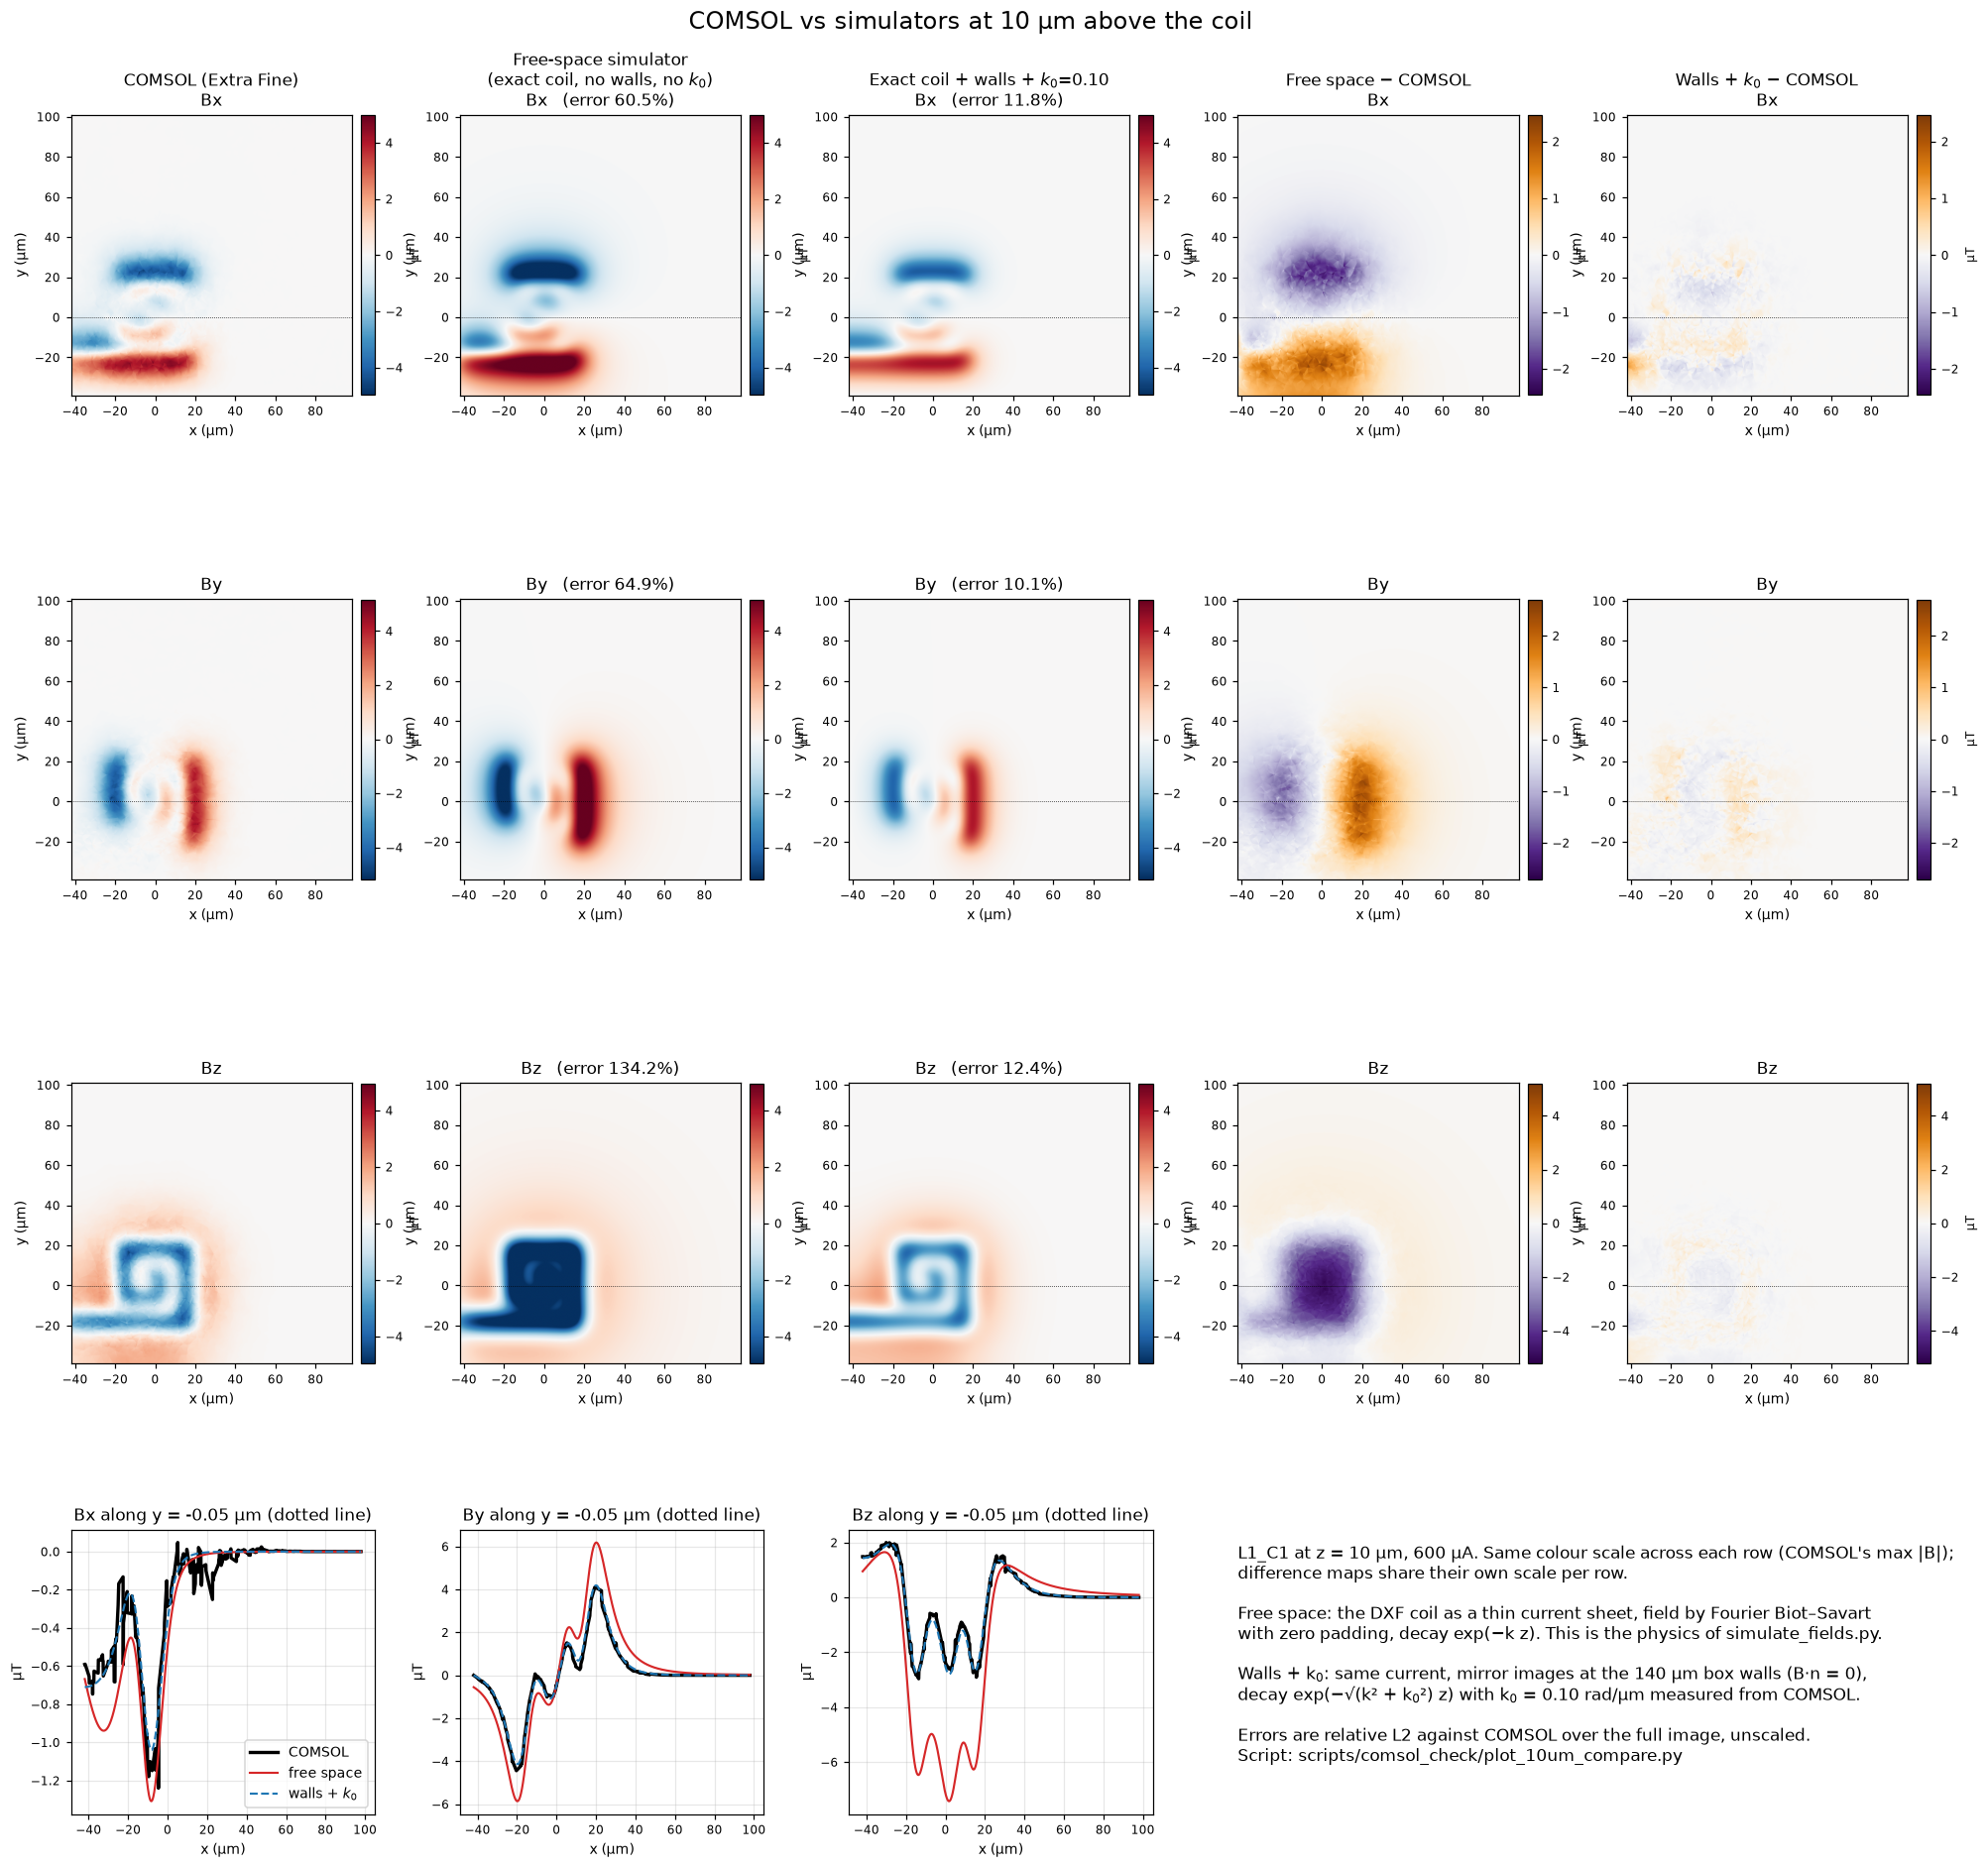
\includegraphics[width=\textwidth]{cm_compare_10um}
\caption{\code{L1_C1} at 10\um. First column: COMSOL. Second: our free-space physics with the exact coil. Third: the same
with walls and $k_0$. Last two columns: the differences. Bottom: cuts through the middle.}
\label{fig:cm_compare}
\end{figure}

\section{Why $k_0$ cannot be physics}

Here is the argument, in two steps you can say out loud.

\textbf{Step 1.} In air there is no current. A static magnetic field in a region with no current must satisfy Laplace's
equation, $\nabla^2B=0$. That forces the decay $e^{-kz}$ and nothing else. COMSOL's field instead satisfies
$\nabla^2B\approx k_0^2\,B$.

\textbf{Step 2.} Amp\`ere's law says the curl of $B$ is the current: $\nabla\times B=\mu_0J$. In empty air $J=0$, so the
curl must be zero. We can test this on COMSOL's own numbers, with no model of ours involved. The horizontal parts of
the curl are
\[
(\nabla\times B)_u=\frac{\partial B_z}{\partial v}-\frac{\partial B_v}{\partial z},\qquad
(\nabla\times B)_v=\frac{\partial B_u}{\partial z}-\frac{\partial B_z}{\partial u}.
\]
The slopes along the plane come from one plane. The slopes in $z$ come from two planes 1\um\ apart:

\begin{code*}{comsol_check/ampere_test.py}
    dzB = [np.real(np.fft.ifft2(b - a))[:N, :N]/dz for a, b in zip(F1, F2)]
    dvBz = np.real(np.fft.ifft2(1j*KV*Fm[2]))[:N, :N]
    duBz = np.real(np.fft.ifft2(1j*KU*Fm[2]))[:N, :N]
    cu = dvBz - dzB[1]
    cv = dzB[0] - duBz
\end{code*}

In each of the last two lines, two terms should cancel exactly. The table gives what is left, as a fraction of the
size of the terms:

\begin{center}
\begin{tabular}{lccc}
\toprule
Between planes & COMSOL & Exact physics (control) & Our model with $k_0=0.10$ \\
\midrule
2 and 3\um & 0.27 & 0.011 & 0.25 \\
3 and 4\um & 0.33 & 0.010 & 0.30 \\
6 and 7\um & 0.41 & 0.007 & 0.44 \\
9 and 10\um & 0.52 & 0.004 & 0.57 \\
\bottomrule
\end{tabular}
\end{center}

The control column runs the \emph{same} estimate on a field from exact physics and gets about 1\%, so the estimate
itself is sound. COMSOL's curl is 27--52\% of the terms that should cancel. In other words, COMSOL's solution has
current flowing in empty air. It runs opposite to the coil current beneath it, like a screening current.

\begin{figure}[H]
\centering
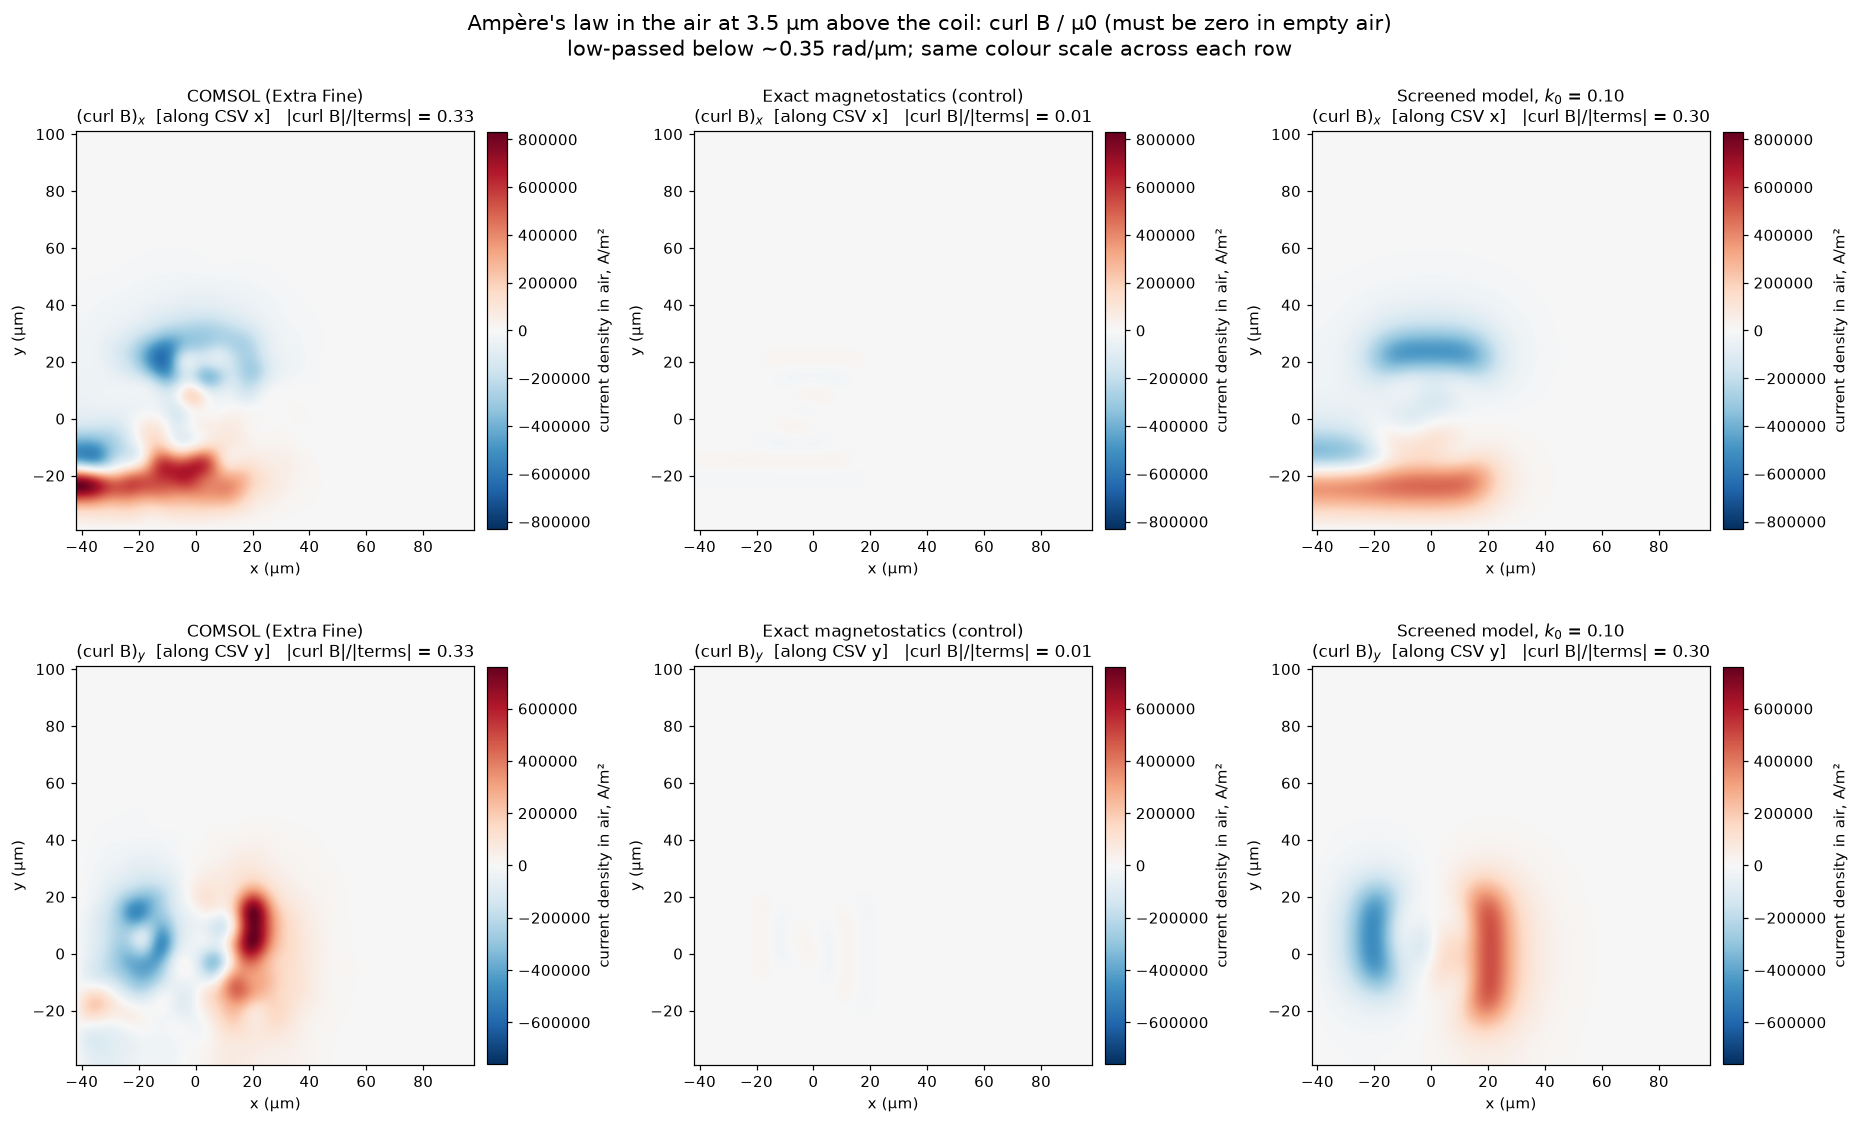
\includegraphics[width=\textwidth]{cm_ampere_air_current}
\caption{The curl of $B$ in the air at 3.5\um, which must be zero. Left: COMSOL. Middle: exact physics. Right: our model
with $k_0$, which reproduces COMSOL's pattern.}
\label{fig:cm_ampere}
\end{figure}

\begin{keyidea}[$k_0$ is not physics]
The air in the model has no conductivity and the study is stationary, so no real current can flow there. And $k_0$ gets
\emph{larger} on the finer mesh (0.12--0.17). A physical effect would not depend on the mesh, and a discretisation
error would shrink on a finer one. So this is a property of how the model was solved.
\end{keyidea}

\begin{careful}[What is not known]
The cause is not established. The candidates are: the iterative solver stopped with an error that is smooth in space;
a regularisation term in the formulation that acts like a weakly screening medium; or a setting in the model file that
the report does not show. One re-solve with a direct solver would separate them. It has been suggested to Hari and has
not been done. The IC coil comes from a different model, for which we have no report; its exports show the same
signature with $k_0\approx0.07$--0.095.
\end{careful}

\section{Is our own simulator right?}

Finding a fault in COMSOL does not prove that we are right. So the simulator was checked against a method that shares
nothing with it: adding up the Biot--Savart law directly along 81 thin filaments of a square loop.

\begin{center}
\begin{tabular}{lccccc}
\toprule
Height & 0.5\um & 1\um & 3\um & 10\um & 20\um \\
\midrule
Simulator against direct Biot--Savart ($B_z$) & 0.54\% & 0.44\% & 0.36\% & 0.74\% & 1.98\% \\
\bottomrule
\end{tabular}
\end{center}

Under 1\% up to 10\um. The rise at 20\um\ has a known cause: the Fourier transform treats the canvas as repeating, and
the loop's far field wraps around. The lesson for high standoffs is to keep the padding generous.

\section{Mesh noise, measured directly}

The same coil on two meshes is two noisy pictures of one true field. Their difference shows the noise:

\begin{center}
\begin{tabular}{lcccc}
\toprule
Frequency band at 0.5\um\ (rad/\um) & below 1 & 1 to 2 & 2 to 2.9 & above 2.9 \\
\midrule
Difference between the meshes, relative & 0.02--0.05 & 0.1--0.2 & about 1.0 & about 1.4 \\
\bottomrule
\end{tabular}
\end{center}

Two independent noise images differ by $\sqrt2\approx1.41$ times one of them. So above 2.9\,rad/\um\ both exports are
pure noise. This is the second confirmation of the noise edge promised in Chapter~\ref{ch:limits}, by a route that
uses no Maxwell equations.

\section{The switch in our simulator}

The simulator can imitate COMSOL's decay if asked. It is one extra term in the exponent:

\begin{code*}{simulate_fields.py}
        decay = 0.5 * MU0_UT * np.exp(-k * z_ref
                                      - np.sqrt(k ** 2 + k0 ** 2) * (z - z_ref))
\end{code*}

Up to the reference plane \code{z_ref} (0.5\um) the decay is the physical $e^{-kz}$. Above it, the rate is
$\sqrt{k^2+k_0^2}$. The default says what we think of it:

\begin{code*}{simulate_fields.py}
    decay_k0=0.0,           # rad/um; nonzero only mimics COMSOL, not physics
\end{code*}

Chapter~\ref{ch:ten_results} uses this switch for one experiment.

\section{The decision}

\begin{center}
\small
\begin{tabularx}{\textwidth}{>{\raggedright\arraybackslash}p{4.6cm}X}
\toprule
Option & What it means \\
\midrule
Add $k_0$ to the simulator and the solvers & COMSOL scores at 5--12\um\ become meaningful, but every model learns a
numerical artefact that a real QDM does not have \\
\textbf{Keep free space} (chosen, 14 November) & Train and test on physically correct data, and report COMSOL above about
4\um\ as a second check with this chapter as the warning \\
Ask for a corrected re-solve & The clean fix; done for L1\_C1 on 14--16 November, and it removed $k_0$ (next section) \\
\bottomrule
\end{tabularx}
\end{center}

\section{Confirmed: the solver tolerance (17 November)}

We asked for one re-solve with a tighter solver. The direct solver could not be used: on this model it stops with
``relative error $1.1\times10^{4}$, returned solution is not converged'', which is what a singular system does (the
vector-potential formulation has no gauge fixing). So Ritaban re-ran the iterative solver with its relative tolerance
tightened to $10^{-8}$, same model, same mesh, and exported L1\_C1 at 0.5, 3 and 10\um.

\begin{figure}[h]
\centering
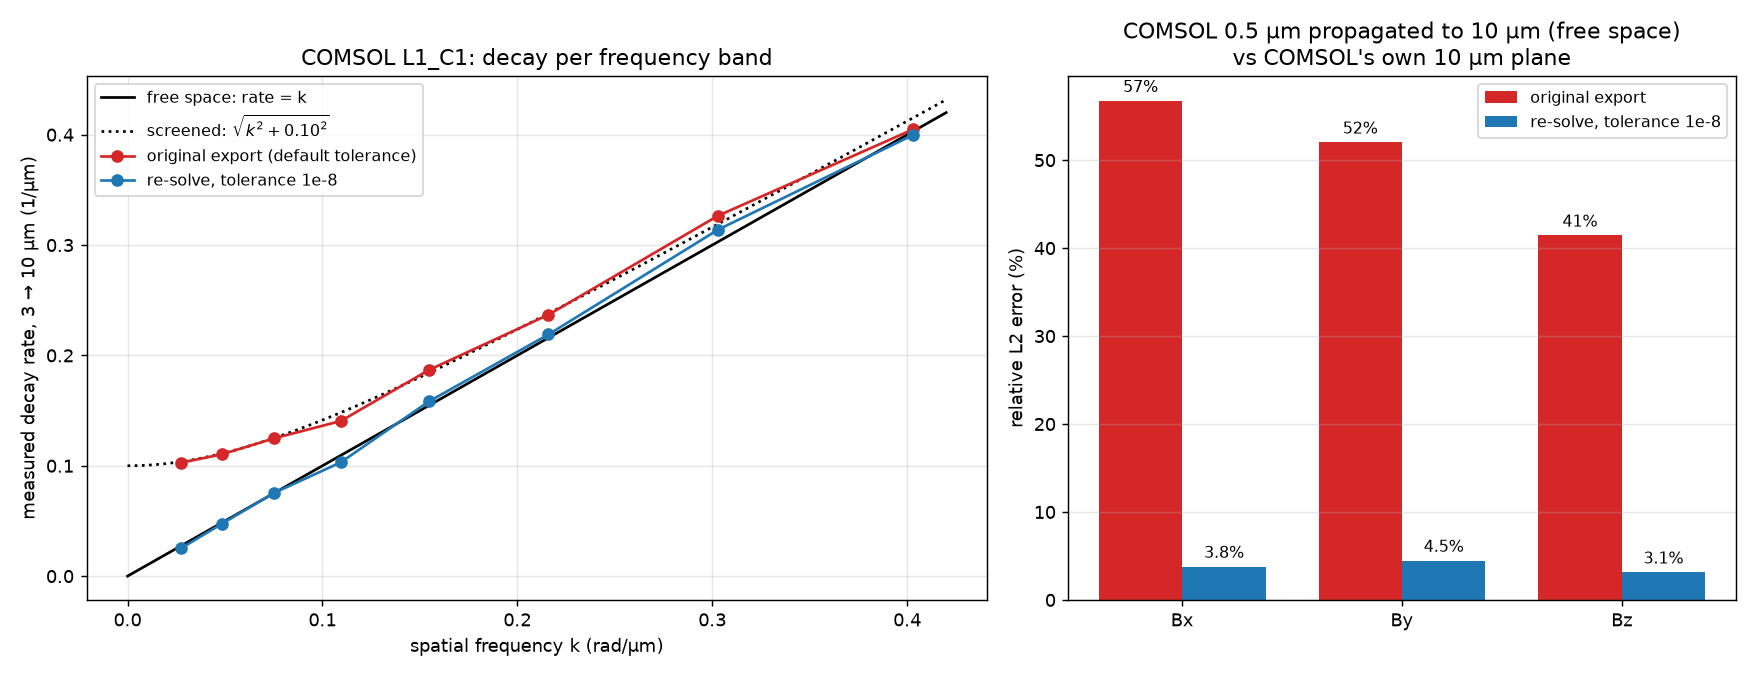
\includegraphics[width=\textwidth]{cm_tolerance_resolve}
\caption{Left: decay rate per frequency band between 3 and 10\um. The original export (red) follows the screened law
$\sqrt{k^2+0.10^2}$; the re-solve (blue) follows free space, rate $=k$. Right: COMSOL's own 0.5\um\ field
propagated to 10\um\ in free space, against COMSOL's 10\um\ plane.}
\end{figure}

\begin{center}
\small
\begin{tabular}{lcc}
\toprule
Check (Bx / By / Bz) & Original export & Re-solve, tolerance $10^{-8}$ \\
\midrule
0.5\um\ propagated to 10\um, against COMSOL 10\um & 57 / 52 / 41\% & \textbf{3.8 / 4.5 / 3.1\%} \\
Our exact-coil simulator (free space) at 10\um & 65 / 58 / 129\% & \textbf{3.2 / 3.2 / 9.3\%} \\
Our exact-coil simulator (free space) at 3\um & 14 / 13 / 25\% & 9.5 / 8.7 / 8.5\% \\
Extra decay $k_0$ & $\approx 0.10$ rad/\um & none \\
\bottomrule
\end{tabular}
\end{center}

\begin{keyidea}[What the re-solve settles]
The extra decay was the default solver tolerance. With a tight tolerance COMSOL obeys free-space magnetostatics, and our
simulator matches it to a few per cent at 10\um. The original exports were off by 39--58\% of the correct field at 10\um\ (60--120\% if the
difference is divided by the original export instead, which is weaker), 9--20\% at 3\um\ and 3--8\% at 0.5\um. Only L1\_C1 at three heights has been re-solved so far; every other COMSOL file still
needs a re-export before it can serve as a clean test.
\end{keyidea}

\section{And Amp\`ere's law? Answered on a single plane}

The re-solve has only three planes (0.5, 3, 10\um), so the test with planes 1\um\ apart cannot be repeated. It does
not need to be. Because $\mathbf{B} = \nabla\times\mathbf{A}$, $\nabla\cdot\mathbf{B}=0$ always, and each Fourier
mode $\mathbf{B}\propto e^{i\mathbf{k}\cdot\mathbf{r}-\gamma z}$ obeys
\begin{equation}
B_z = \frac{i\,\mathbf{k}\cdot\mathbf{B}_t}{\gamma}.
\end{equation}
Amp\`ere's law, $\nabla\times\mathbf{B}=0$, holds if and only if $\gamma = k$. So on one plane the ratio
$R(k) = B_z/[\,i\,\mathbf{k}\cdot\mathbf{B}_t/k\,]$ must be 1 in every band. A screened field gives
$k/\sqrt{k^2+k_0^2}$.

\begin{figure}[h]
\centering
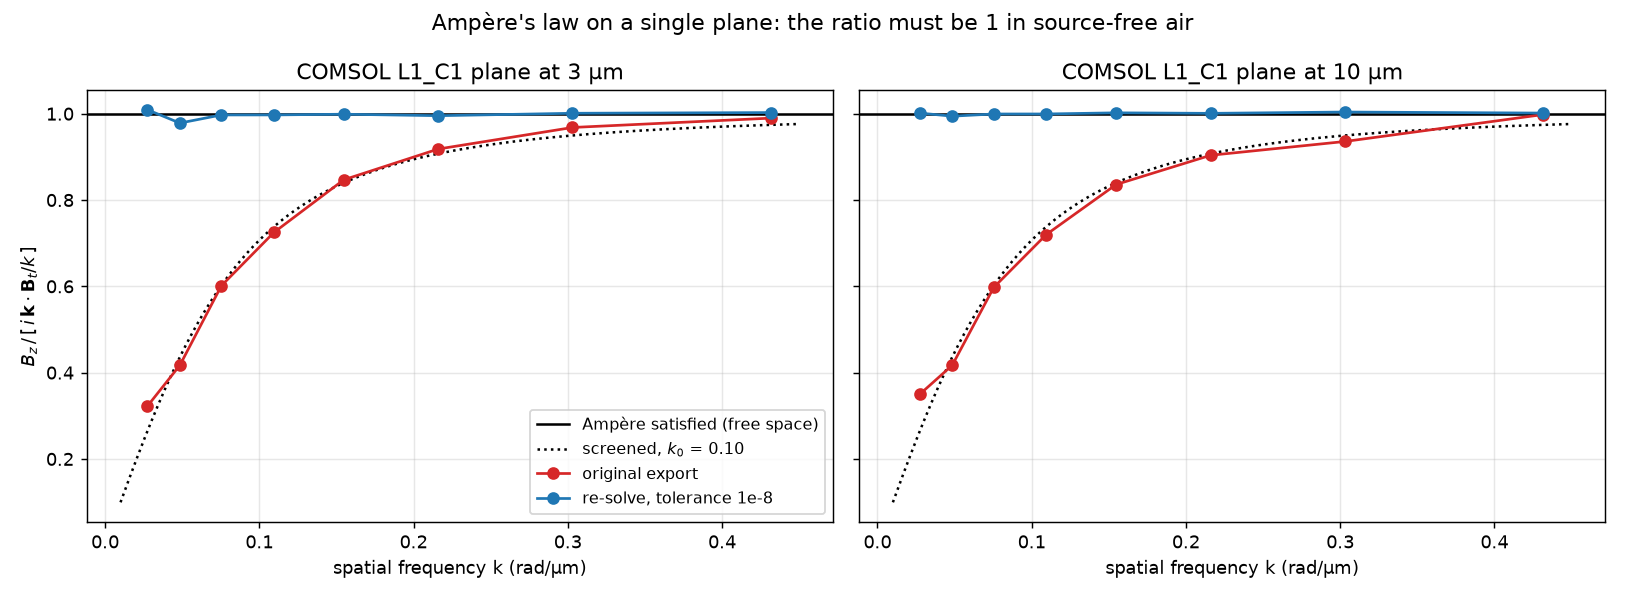
\includegraphics[width=\textwidth]{cm_ampere_single_plane}
\caption{The single-plane Amp\`ere test. The original export (red) follows the screened law with $k_0=0.10$; the
re-solve (blue) gives 1.00 in every band at 3 and at 10\um.}
\end{figure}

\begin{keyidea}[The answer]
The original export had current flowing in empty air because of a loose solver tolerance. With the tolerance at
$10^{-8}$ the field satisfies Amp\`ere's law to 1--2\% in the lowest bands and better than 0.5\% above. The air current
was numerical, and it is gone.
\end{keyidea}

\section{Seeing it: three versions of the same coil}

Numbers like ``58\% off'' are easy to read past. So here is the same coil, \code{L1_C1}, three ways:
\begin{itemize}
\item \textbf{Original export}: what we used for every COMSOL score until 17 November, solved with COMSOL's default
tolerance.
\item \textbf{Re-solve}: the same model and mesh, solved with the tolerance tightened to $10^{-8}$.
\item \textbf{Our simulator}: the physics of our training data (Chapter~\ref{ch:simulation}): a thin current sheet at
$z=0$, the thin-sheet Biot--Savart formulas, and decay $e^{-kz}$. The current is the exact coil from the drawing
(\code{Gemetry_C1.dxf}), 600\,\textmu A, spread over each 2\um\ wire by a conduction solve. Nothing is fitted: no scale, no
height, no offset. Only the direction of the current is read from the data.
\end{itemize}

\begin{sidewaysfigure}
\centering
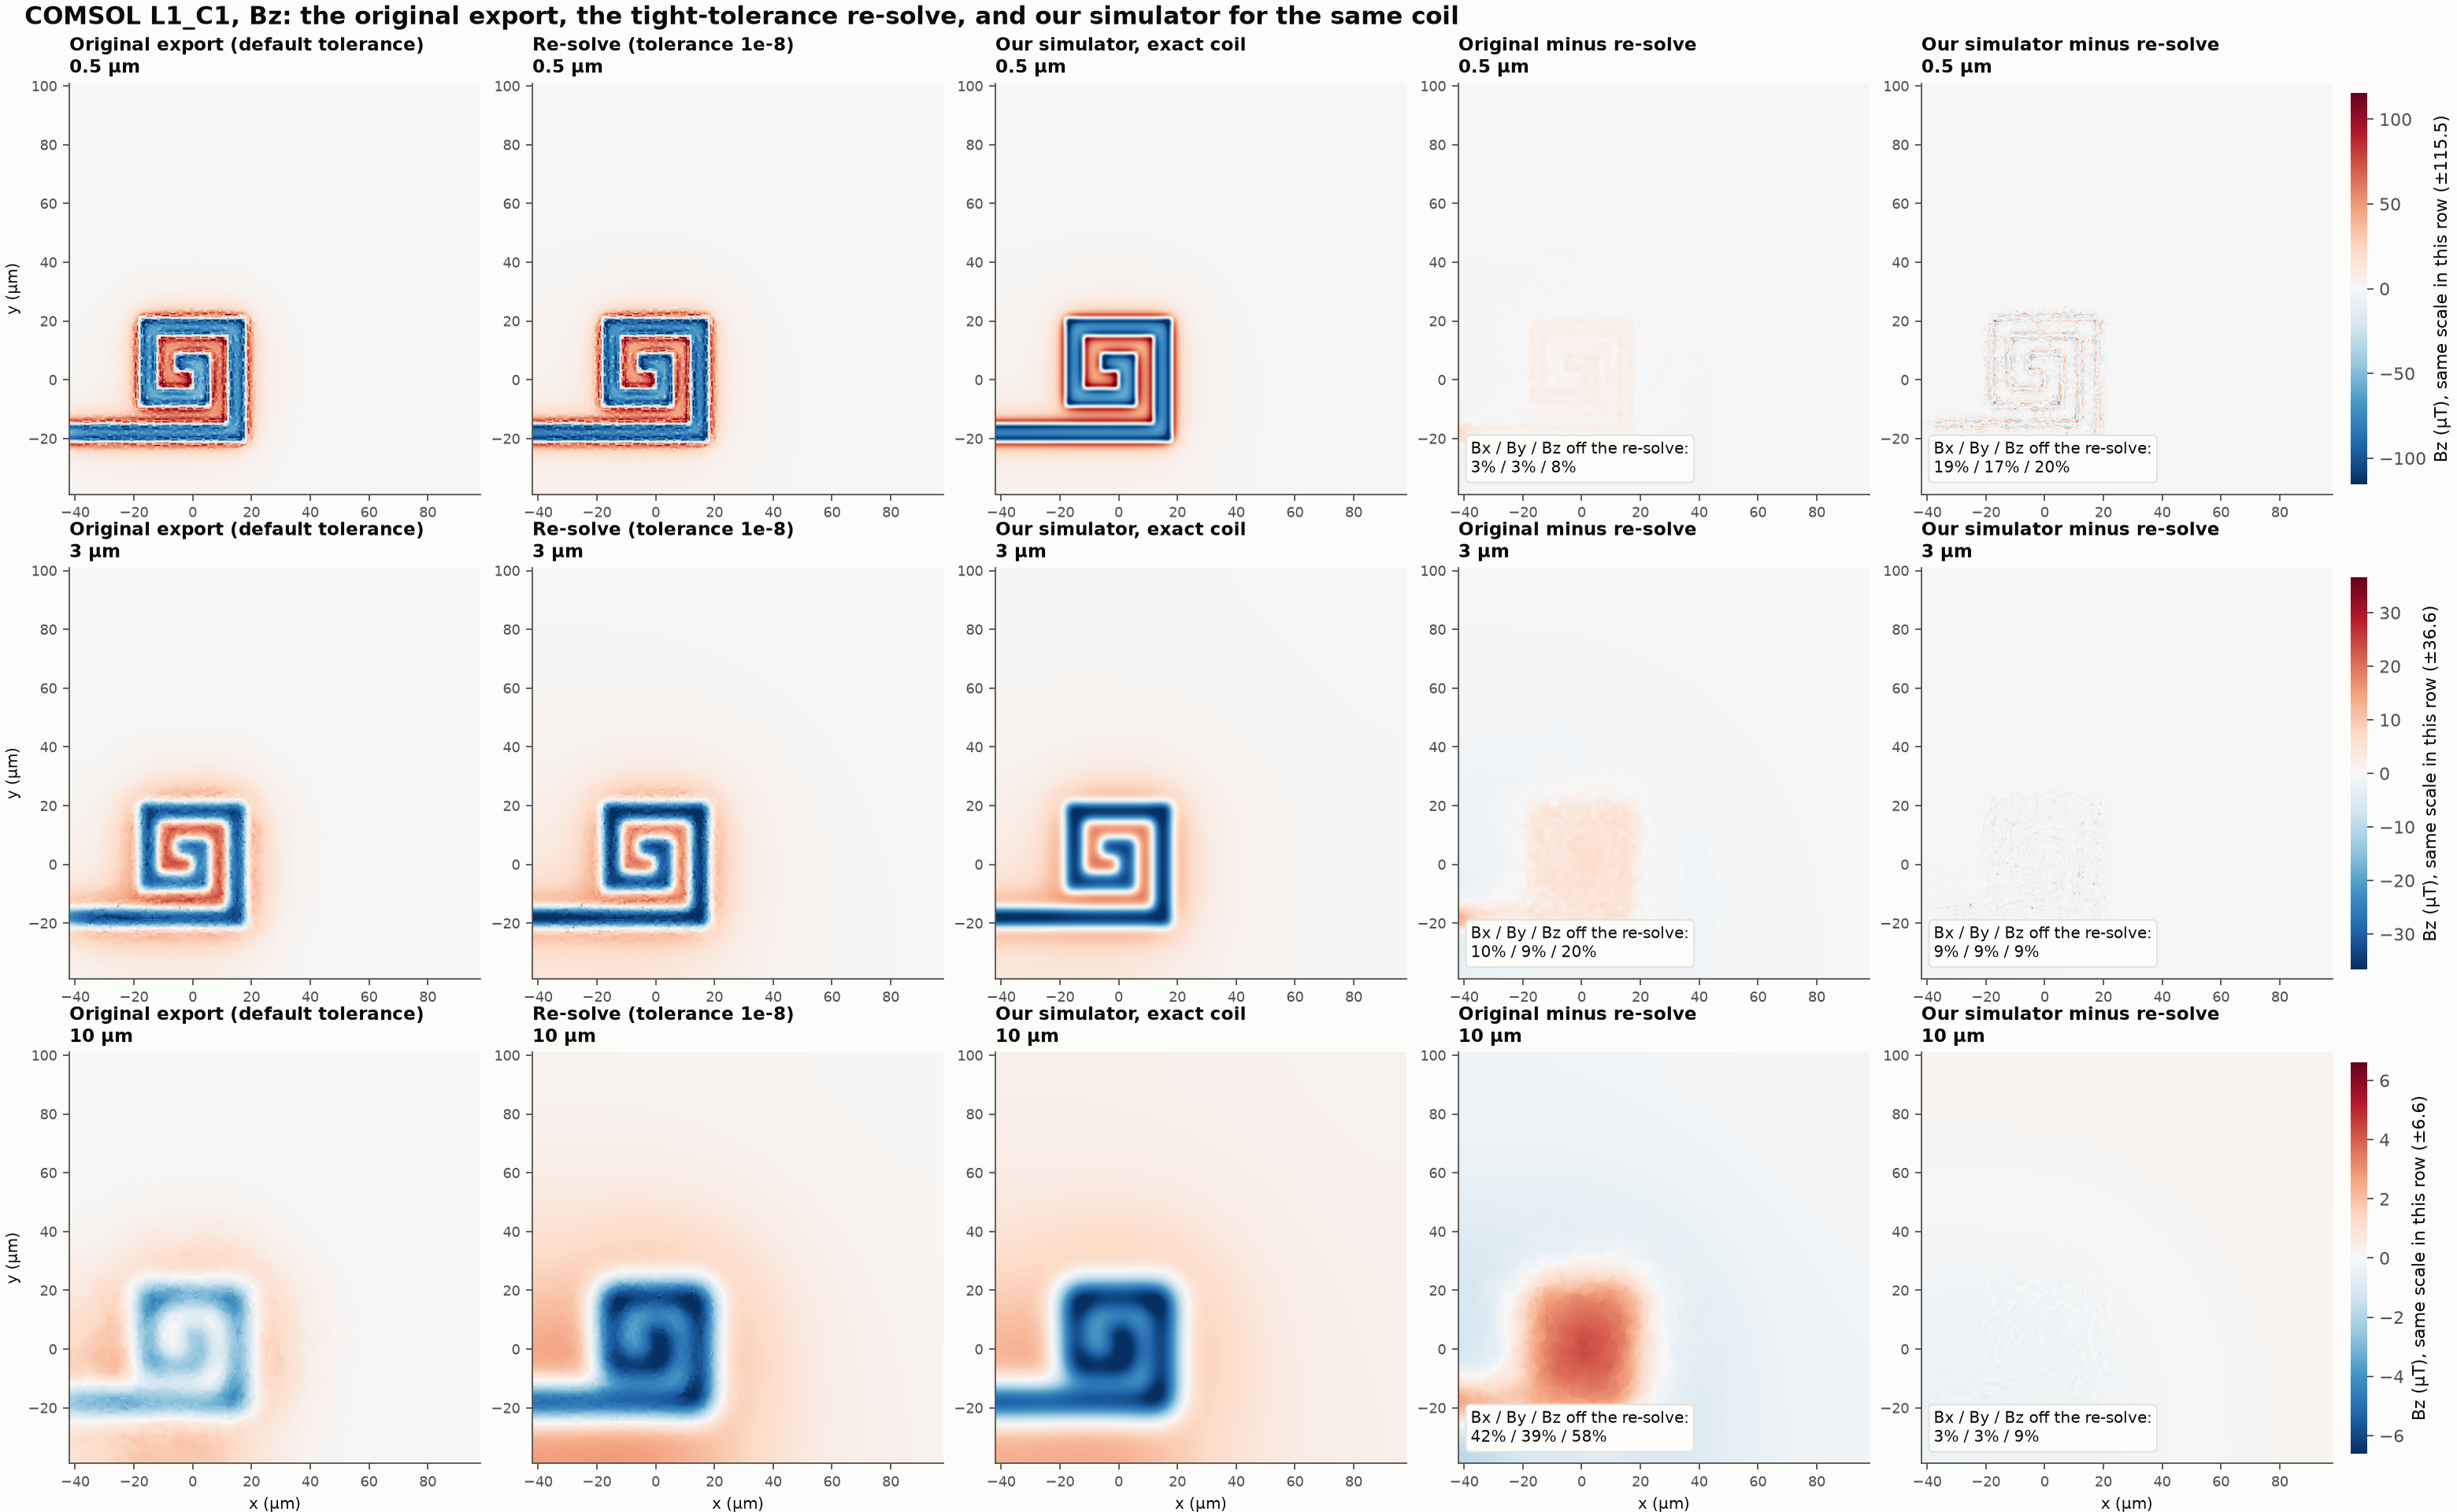
\includegraphics[width=\textheight]{cm_resolve_vs_old_maps}
\caption{$B_z$ of the three versions at 0.5, 3 and 10\um, and the differences from the re-solve. Each row has one colour
scale, so a lighter panel really is a weaker field.}
\label{fig:cm_three_maps}
\end{sidewaysfigure}

Read Figure~\ref{fig:cm_three_maps} row by row.
\begin{itemize}
\item \textbf{At 0.5\um} all three show the same spiral. The original and the re-solve differ by 3--8\%. Our simulator
differs from the re-solve by 17--20\%, but look at its difference panel: the error is a fine speckle along every wire
edge. That is COMSOL's mesh noise, which Chapter~\ref{ch:limits} measured at 14--18\% of the 0.5\um\ target. A clean
simulator cannot reproduce it, and should not.
\item \textbf{At 3\um} the original is already a little weak inside the coil (20\% off in $B_z$); our simulator is 9\%
off, again mostly speckle.
\item \textbf{At 10\um} the original has lost almost half its strength: its difference panel is one large smooth blob.
Our simulator's difference panel is nearly blank: 3 / 3 / 9\% off.
\end{itemize}

\begin{figure}[H]
\centering
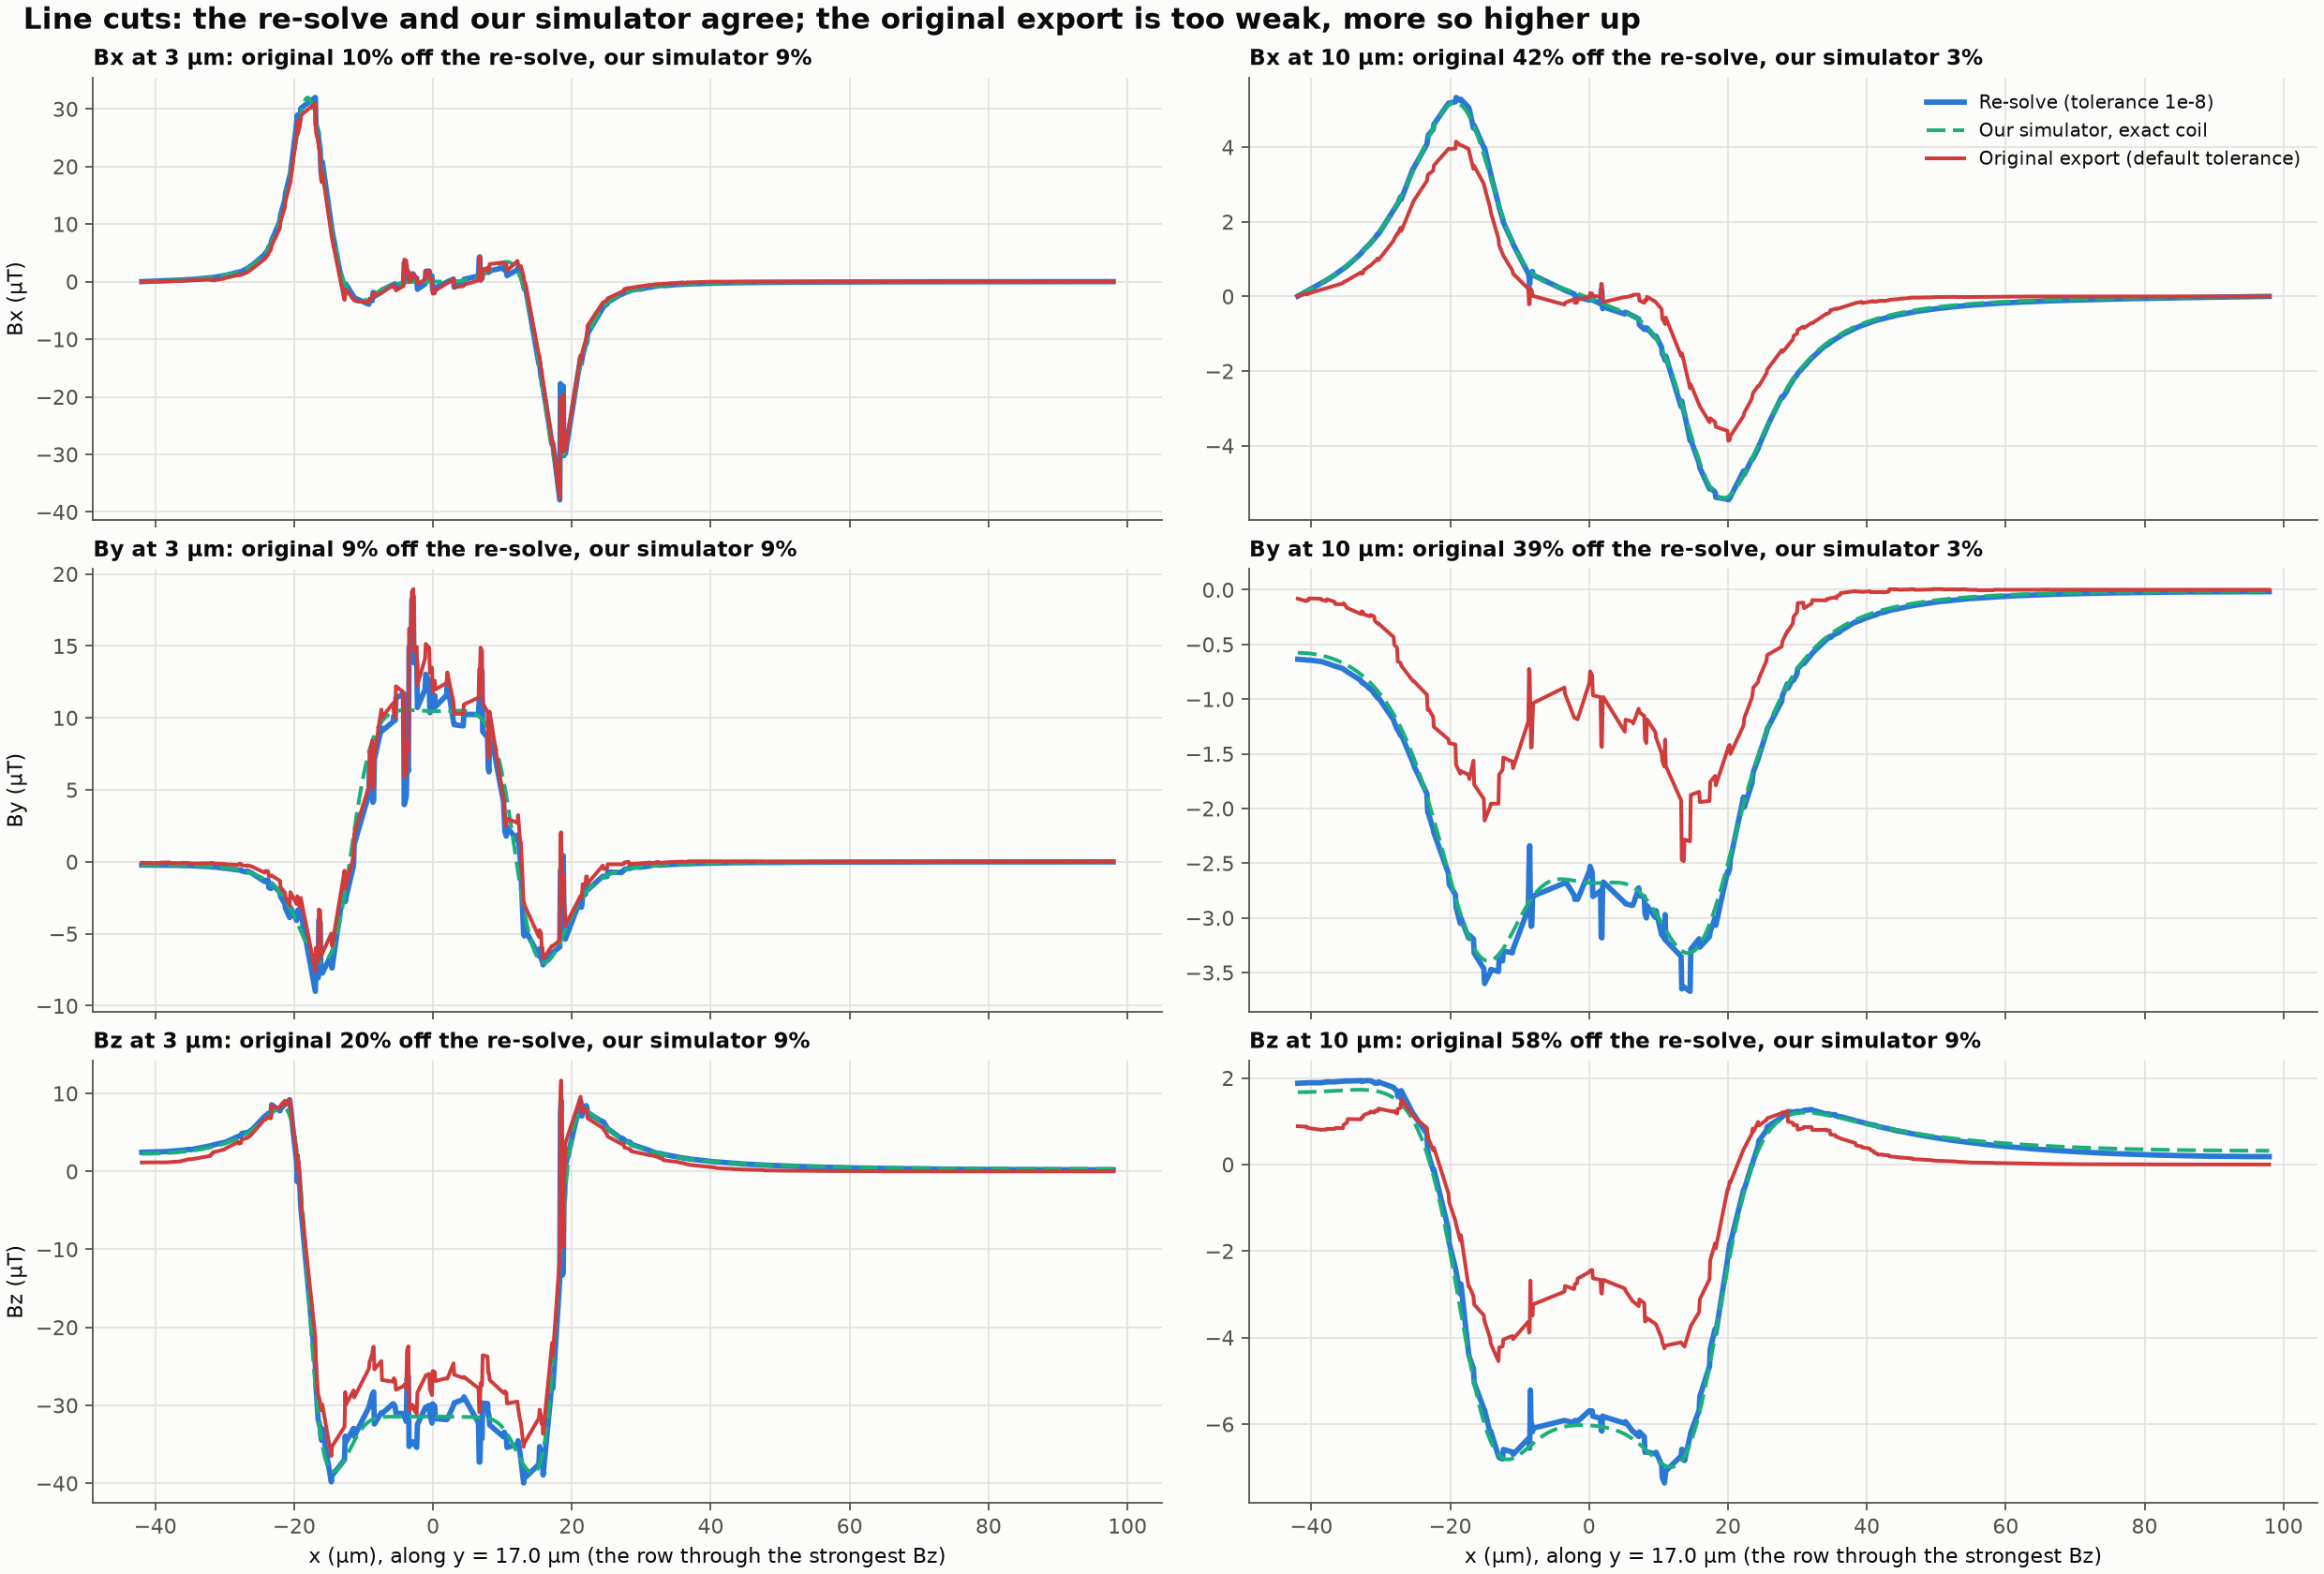
\includegraphics[width=\textwidth]{cm_resolve_vs_old_linecut}
\caption{A cut through the coil at 3\um\ (left) and 10\um\ (right), all three components. Blue: re-solve. Green
dashed: our simulator. Red: original export.}
\label{fig:cm_three_cuts}
\end{figure}

The line cuts make the point with no colour scale to argue about. At 3\um\ the three curves almost sit on each other.
At 10\um\ the green dashed line of our simulator lies on the blue re-solve, and the red original sits well inside both:
too weak, in every component.

\subsection*{Why an early-stopped solve damages exactly this}

COMSOL turns the physics into one enormous linear system, $A\mathbf{u}=\mathbf{f}$, with millions of unknowns. It does
not solve it in one go. An iterative solver starts from a guess and improves it step by step, and it stops once the
leftover mismatch is a small enough fraction of $\mathbf{f}$. That fraction is the tolerance.

Two facts then explain everything you see above.
\begin{enumerate}
\item \textbf{The error left behind is smooth.} Iterative solvers remove sharp, local errors quickly; broad, smooth
errors are the last to go. So when the solver stops early, what is left is a smooth error. In the field, smooth means
broad structure: low spatial frequencies $k$.
\item \textbf{Higher up, the field \emph{is} broad structure.} Fine detail decays as $e^{-kz}$, so the higher you go, the
more of what is left is broad. The right panel of Figure~\ref{fig:cm_three_why} measures it: the share of the field's
energy below $k=0.1$\,rad/\um\ is 2\% at 0.5\um, 11\% at 3\um\ and 68\% at 10\um.
\end{enumerate}
A smooth error is invisible near the coil, where almost nothing is broad, and dominant at 10\um, where almost everything
is.

\begin{sidewaysfigure}
\centering
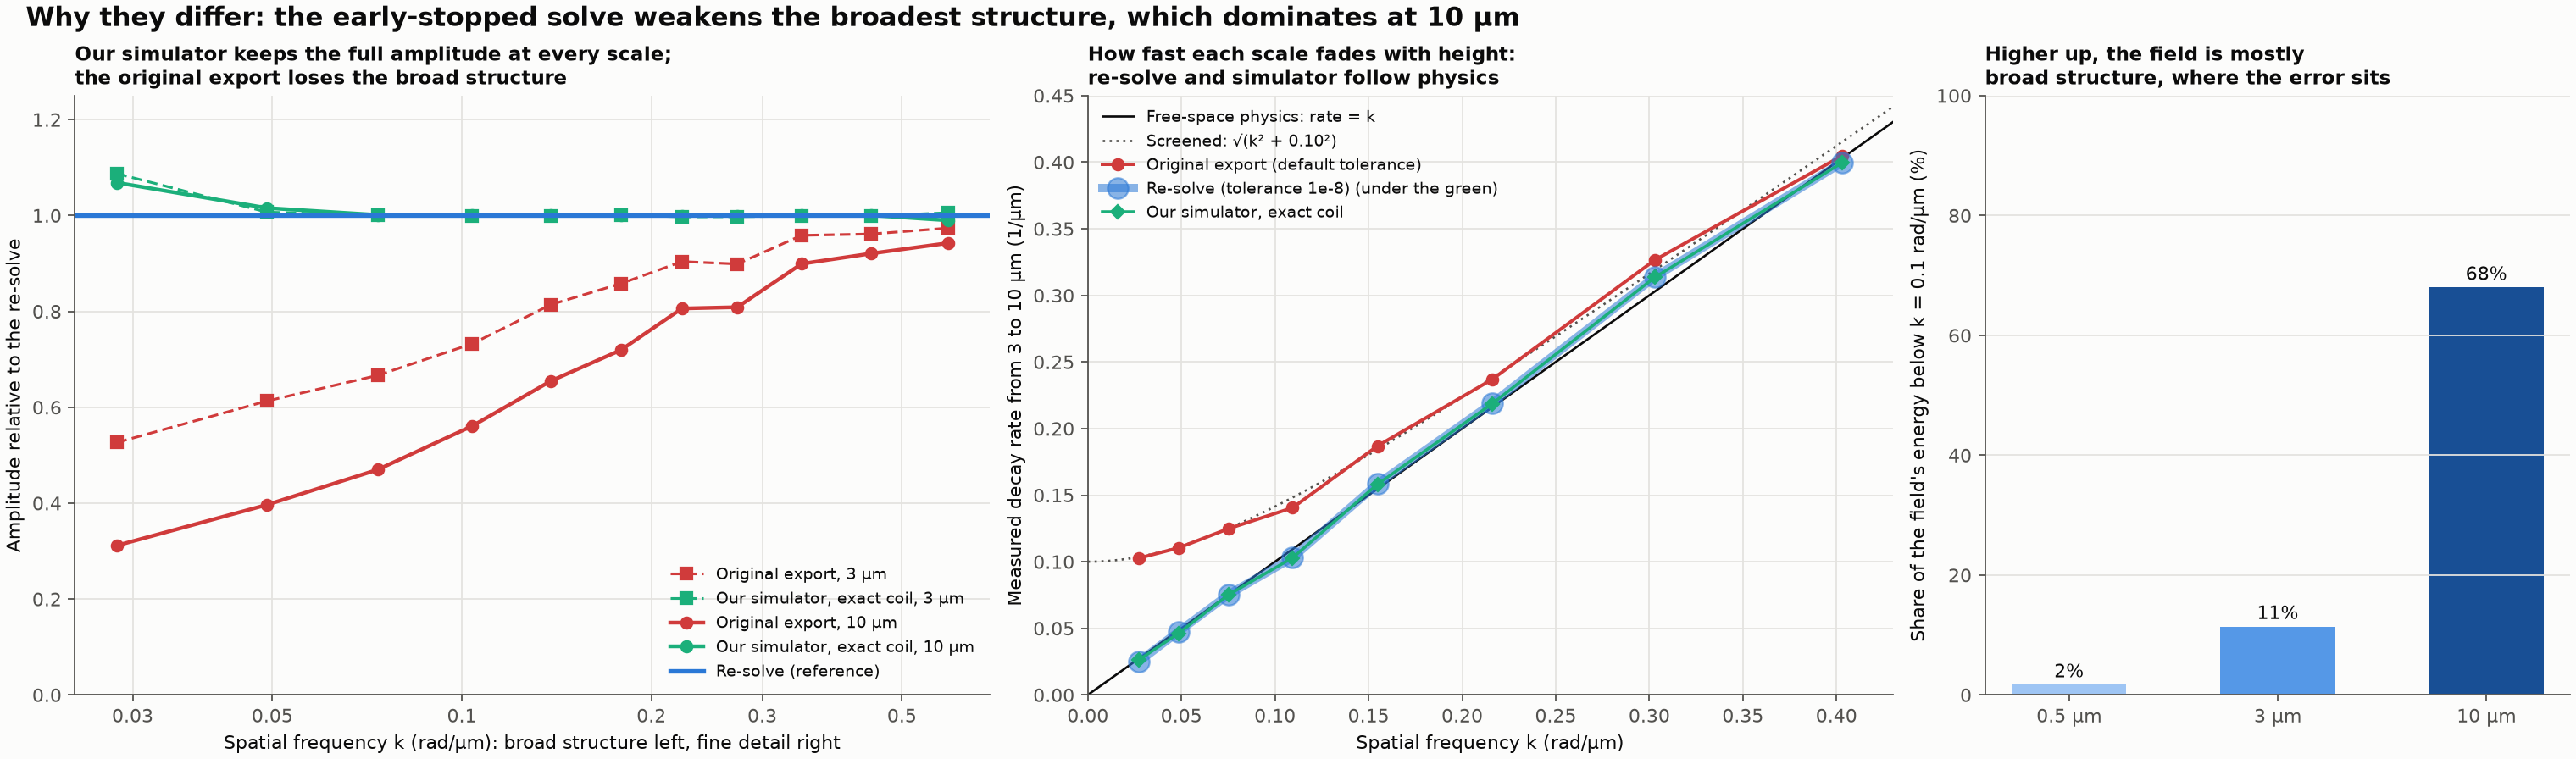
\includegraphics[width=\textheight]{cm_resolve_vs_old_why}
\caption{Left: amplitude of each version relative to the re-solve, per spatial frequency. Middle: how fast each
frequency fades between 3 and 10\um; free-space physics says the rate equals $k$. Right: how much of the field is broad
structure at each height.}
\label{fig:cm_three_why}
\end{sidewaysfigure}

\begin{itemize}
\item \textbf{Left:} the original export (red) keeps more than 90\% of the fine detail but only about 30\% of the broadest
structure at 10\um, and about 50\% at 3\um. Our simulator (green) stays at 1.0 at every scale; only the broadest band is
about 8\% high, where the coil's leads and the box walls matter most.
\item \textbf{Middle:} the original fades on the screened curve $\sqrt{k^2+0.10^2}$ of Section~\ref{sec:cm_decay}. The
re-solve and our simulator both fade at exactly $k$, as physics requires, and lie on top of each other.
\end{itemize}

\begin{center}
\small
\begin{tabular}{lccc}
\toprule
Off the re-solve ($B_x$ / $B_y$ / $B_z$) & 0.5\um & 3\um & 10\um \\
\midrule
Original export & 3 / 3 / 8\% & 10 / 9 / 20\% & 42 / 39 / 58\% \\
Our simulator, exact coil & 19 / 17 / 20\% & 9 / 9 / 9\% & \textbf{3 / 3 / 9\%} \\
\bottomrule
\end{tabular}
\end{center}

\begin{keyidea}[Where our simulator lies]
Next to the correctly solved field. Higher up, where COMSOL's mesh noise has decayed away, our simulator matches it to a
few per cent with nothing fitted. Near the coil the remaining difference is mostly mesh noise in COMSOL. The physics
used for every training set in this project was right; it was the old COMSOL export that was off.
\end{keyidea}

\begin{careful}[One modelling detail]
The figures close the coil's leads through the box walls, as COMSOL does. Our training layouts instead close every
loop with a rail outside the image. With plain zero padding and the leads simply ending at the image edge, the
simulator is 7 / 15 / 25\% off the re-solve at 10\um: the missing return current adds a field near the edge. That is a
statement about how this coil's leads are modelled, not about the physics.
\end{careful}

\textbf{What it changed for the results.} Every COMSOL score at 10\um\ in Chapter~\ref{ch:ten_results} used the original
export as input. On the re-solved \code{L1_C1}, MAGIC-UNet's 10\um\ error falls from 60.4\% to 26.2\%
(Section~\ref{sec:resolved}).

\begin{defend}[If your professor asks: why trust the re-solve and not the original?]
Because three independent checks agree with it and not with the original: it fades at exactly the free-space rate, it
satisfies Amp\`ere's law in empty air on a single plane, and it matches our simulator of the exact coil to 3--9\% at
10\um\ with nothing fitted. The original fails all three, and the only thing changed between them is the solver
tolerance.
\end{defend}

\begin{defend}[If your professor asks: how can you say COMSOL is wrong?]
COMSOL is not wrong; its default solver setting was too loose for the weak far field, and the re-solve with a tight
tolerance agrees with free-space physics to a few per cent. Before the re-solve: not wrong everywhere: near the coil it is fine, and at 3\um\ the effect is a few per cent in the measured band. But
above about 4\um\ its field in the air violates Amp\`ere's law by 27--52\%, where exact physics gives 1\% in the same
test. Empty air cannot carry current. Our simulator matches an independent Biot--Savart calculation to under 1\%, and
matches COMSOL to 10--12\% at every height once this one term is added.
\end{defend}

\begin{defend}[If your professor asks: why not just add $k_0$ and match the data?]
Because it would teach the network something that is not true of a real measurement. Chapter~\ref{ch:ten_results} shows
what the term does to a network trained without it: tens of points. A network trained \emph{with} it would lose those
points on a real instrument instead.
\end{defend}
